\begin{intersong}
    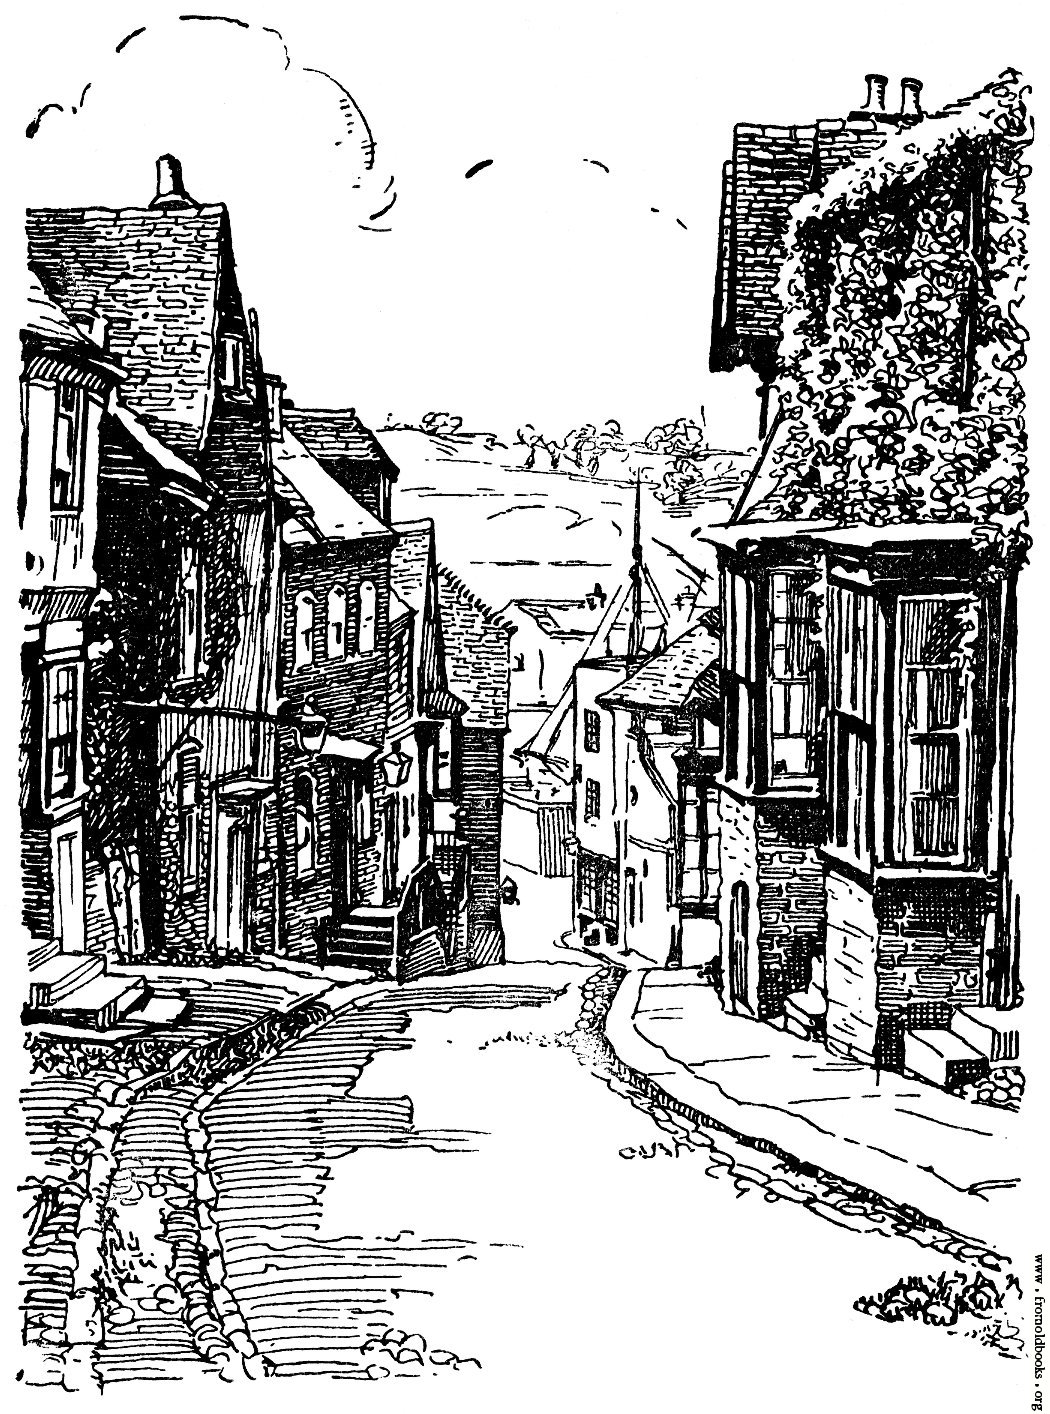
\includegraphics[width=0.4\textwidth]{destratenzijdreunen}
\end{intersong}
\beginsong{De straten zij dreunen}
\beginverse*
De straten zij dreunen bij 't schrijden,
Zo koel waait de morgenwind,
Vooraan steeds het vaandel dat wappert,
Vooraan waar het doel zich bevindt.
\endverse
\beginchorus
En schijnt ook daarboven, De hemel zo grauw;
Boven de wolken, Blijft 't eeuwig blauw.
\endchorus
\beginverse*
Wij willen de laagheid verderven,
Wij dromen van trouw en van eer,
De wereld zij mag ons onterven,
Ons stappen zij keren niet weer.
\endverse
\beginverse*
Wij zullen geen roem ons verwerven,
Maar hoog boven laster en haat,
Staat stralend geplant op de scherven,
Het vaandel dat nimmer vergaat.
\endverse
\endsong